% vim:fdl=0
\documentclass[a4paper, 11pt]{article}           %{{{1
% basic packages                                 {{{2
\usepackage[T1]{fontenc}
\usepackage[scaled=0.975]{helvet}
\usepackage[utf8]{inputenc}
\usepackage{amsmath}
\usepackage{lastpage}
\usepackage{graphicx}
\usepackage{xcolor}
\usepackage{listings}                                                           %
\usepackage{multicol}
\usepackage{gensymb}                                                            % \degree \ohm ....
\usepackage{tcolorbox}                                                          % encadrement texte
% ==== MATHS
\usepackage{pgf,tikz}                                                           % dessin
% ==== PROGRAMMATION
\usepackage{xcolor}                                                             %
\usepackage{listings}                                                           %
% listings                                        {{{3
\definecolor{mygreen}{rgb}{0,0.6,0}
\definecolor{mygray}{rgb}{0.5,0.5,0.5}
\definecolor{mymauve}{rgb}{0.58,0,0.82}
\definecolor{deepblue}{rgb}{0,0,0.5}
\definecolor{deepred}{rgb}{0.6,0,0}
\definecolor{deepgreen}{rgb}{0,0.5,0}
\lstset{%
%       backgroundcolor=\color{white},   % choose the background color; you must add \usepackage{color} or \usepackage{xcolor}; should come as last argument
        basicstyle=\footnotesize,        % the size of the fonts that are used for the code
%       breakatwhitespace=false,         % sets if automatic breaks should only happen at whitespace
%       breaklines=true,                 % sets automatic line breaking
%       captionpos=b,                    % sets the caption-position to bottom
        commentstyle=\color{mygreen},    % comment style
%       deletekeywords={type},           % if you want to delete keywords from the given language
%       emph={},                         % Custom highlighting
%       emphstyle=\ttb\color{deepred}    % Custom highlighting style
%       escapeinside={\%*}{*)},          % if you want to add LaTeX within your code
%       extendedchars=true,              % lets you use non-ASCII characters; for 8-bits encodings only, does not work with UTF-8
        frame=shadowbox,                 % adds a frame around the code {single, shadowbox}
%       keepspaces=true,                 % keeps spaces in text, useful for keeping indentation of code (possibly needs columns=flexible)
        keywordstyle=\color{blue},       % keyword style
	language=C,                      % the language of the code {Python, C}
%       morekeywords={*,...},            % if you want to add more keywords to the set
        numbers=left,                    % numbers = (none, left, right)
%       numbersep=5pt,                   % how far the line-numbers are from the code
%       numberstyle=\tiny\color{mygray}, % the style that is used for the line-numbers
%       otherkeywords={self},            % Add keywords here
%       rulecolor=\color{black},         % if not set, the frame-color may be changed on line-breaks within not-black text (e.g. comments (green here))
	rulesepcolor=\color{gray}        % shadowbox color
%       showspaces=false,                % show spaces everywhere adding particular underscores; it overrides 'showstringspaces'
%       showstringspaces=false,          % underline spaces within strings only
%       showtabs=false,                  % show tabs within strings adding particular underscores
%       stepnumber=1,                    % the step between two line-numbers. If it's 1, each line will be numbered
%       stringstyle=\color{mymauve},     % string literal style
%       tabsize=4,                       % sets default tabsize to 2 spaces
%       title=\lstname                   % show the filename of files included with \lstinputlisting; also try caption instead of title
}
%}}}
%}}}

% mise en page                                    {{{2
\addtolength{\voffset}{-1.8cm}
\addtolength{\textheight}{4cm}
\addtolength{\hoffset}{-2.5cm}
\addtolength{\textwidth}{4cm}
\addtolength{\headsep}{-0.5cm}
\usepackage{fancyhdr}
\setlength{\headheight}{14.00pt}
\pagestyle{fancy} % Numérotation des pages
\renewcommand\headrulewidth{1pt}
\renewcommand\footrulewidth{1pt}
\fancyhead[L]{BP SN}
\fancyhead[C]{arduino}
\fancyhead[R]{PIR et LCD}
\fancyfoot[L]{v 1.5 -- JB}
\fancyfoot[C]{\textbf{gestion de l'habitat: detection intrusion}}
\fancyfoot[R]{\thepage/\pageref{LastPage}}
%}}}

% Compteurs:                                     {{{2
\addtocounter{page}{0}
\newcounter{Q}
\newcounter{exoNB}
%}}}

% newcommand                                     {{{2
\newcommand{\objectif}[1]{\textsc{\huge \textbf{Objectif :}\\[2mm] #1} }
\newcommand{\partie}[1]{\textsc{\Large #1} }

\newcommand{\question}{\stepcounter{Q} $\boxed{\arabic{Q}}$ }

\newcommand{\reponse}{
\par\nobreak
\noindent\rule{0pt}{1.5\baselineskip}% Provides a larger gap between the preceding paragraph and the dots
{\noindent\makebox[\linewidth]{\dotfill}\endgraf}% ... dotted lines ...
% \bigskip% Gap between dots and next paragraph
}

\newcommand{\ligne}{\underline{\hspace{ \textwidth}} }
\newcommand{\exo}[1]{\stepcounter{exoNB}\textsc{\Large Exercice \arabic{exoNB} -- #1} }
\newcommand{\EXO}[2]{\stepcounter{exoNB}\textsc{\Large Exercice \arabic{exoNB} -- #1} \hfill \textbf{#2 points}}
\newcommand{\pb}[1] {\stepcounter{exoNB}\textsc{\Large Problème \arabic{exoNB} -- #1} }
\newcommand{\PB}[2] {\stepcounter{exoNB}\textsc{\Large Problème \arabic{exoNB} -- #1} \hfill \textbf{#2 points}}
%}}}

% Longueur:                                      {{{2
\newlength{\longueurA}
\newlength{\longueurB}
\setlength{\parindent}{0pt}
\setlength{\parskip}{2pt}
\renewcommand{\baselinestretch}{1}
%}}}

% Divers                                          {{{2
% listings                                        {{{3
%\definecolor{mygreen}{rgb}{0,0.6,0}
%\definecolor{mygray}{rgb}{0.5,0.5,0.5}
%\definecolor{mymauve}{rgb}{0.58,0,0.82}
%\definecolor{deepblue}{rgb}{0,0,0.5}
%\definecolor{deepred}{rgb}{0.6,0,0}
%\definecolor{deepgreen}{rgb}{0,0.5,0}
%\lstset{%
%        backgroundcolor=\color{white},   % choose the background color; you must add \usepackage{color} or \usepackage{xcolor}; should come as last argument
%        basicstyle=\footnotesize,        % the size of the fonts that are used for the code
%        breakatwhitespace=false,         % sets if automatic breaks should only happen at whitespace
%        breaklines=true,                 % sets automatic line breaking
%        captionpos=b,                    % sets the caption-position to bottom
%        commentstyle=\color{mygreen},    % comment style
%        deletekeywords={...},            % if you want to delete keywords from the given language
%        escapeinside={\%*}{*)},          % if you want to add LaTeX within your code
%        extendedchars=true,              % lets you use non-ASCII characters; for 8-bits encodings only, does not work with UTF-8
%        frame=single,                    % adds a frame around the code
%        keepspaces=true,                 % keeps spaces in text, useful for keeping indentation of code (possibly needs columns=flexible)
%        keywordstyle=\color{blue},       % keyword style
%        morekeywords={*,...},            % if you want to add more keywords to the set
%        numbers=left,                    % where to put the line-numbers; possible values are (none, left, right)
%        numbersep=5pt,                   % how far the line-numbers are from the code
%        numberstyle=\tiny\color{mygray}, % the style that is used for the line-numbers
%        rulecolor=\color{black},         % if not set, the frame-color may be changed on line-breaks within not-black text (e.g. comments (green here))
%        showspaces=false,                % show spaces everywhere adding particular underscores; it overrides 'showstringspaces'
%        showstringspaces=false,          % underline spaces within strings only
%        showtabs=false,                  % show tabs within strings adding particular underscores
%        stepnumber=2,                    % the step between two line-numbers. If it's 1, each line will be numbered
%        stringstyle=\color{mymauve},     % string literal style
%        tabsize=4,                       % sets default tabsize to 2 spaces
%        title=\lstname                   % show the filename of files included with \lstinputlisting; also try caption instead of title
%}
%\lstset{%
%        language=Python,                 % the language of the code
%        otherkeywords={self},            % Add keywords here
%        deletekeywords={type},           % if you want to delete keywords from the given language
%        emph={},                         % Custom highlighting
%        emphstyle=\ttb\color{deepred}    % Custom highlighting style
%}
%}}}

% PRL style line                                 {{{3
\newlength{\diamondrulelength}
\setlength{\diamondrulelength}{0.6\textwidth}
\newlength{\diamondrulethickness}
\setlength{\diamondrulethickness}{2pt}
\newcommand{\diamondrule}{\begin{center}\tikz{\fill[black] (0.5\diamondrulelength,0) -- (0,0.5\diamondrulethickness) -- (-0.5\diamondrulelength,0) -- (0,-0.5\diamondrulethickness) -- cycle;}\end{center}}
%}}}

% fixed with tabular                             {{{3
\usepackage{array}
\newcolumntype{L}[1]{>{\raggedright\let\newline\\\arraybackslash\hspace{0pt}}m{#1}}
\newcolumntype{C}[1]{>{\centering\let\newline\\\arraybackslash\hspace{0pt}}m{#1}}
\newcolumntype{R}[1]{>{\raggedleft\let\newline\\\arraybackslash\hspace{0pt}}m{#1}}
%}}}

%}}}
%}}}

\begin{document}
\sffamily
\hfill Nom : {\noindent\makebox[5cm]{\dotfill}\endgraf}
\objectif{Détecteur de proximité \& écran LCD} \\

\partie{Materiel}                         %{{{1
\begin{multicols}{2}
Arduino Board *1 \\
USB Cable *1 \\
I2C 1602 LCD *1 \\
PIR Motion Sensor*1 \\
Red M5 LED*1 \\
220$\Omega$ Resistor *1 \\
Breadboard *1 \\
Breadboard Jumper Wires \\
Male to Female Dupont Line
\end{multicols}
\begin{figure}[!h]
\begin{center}
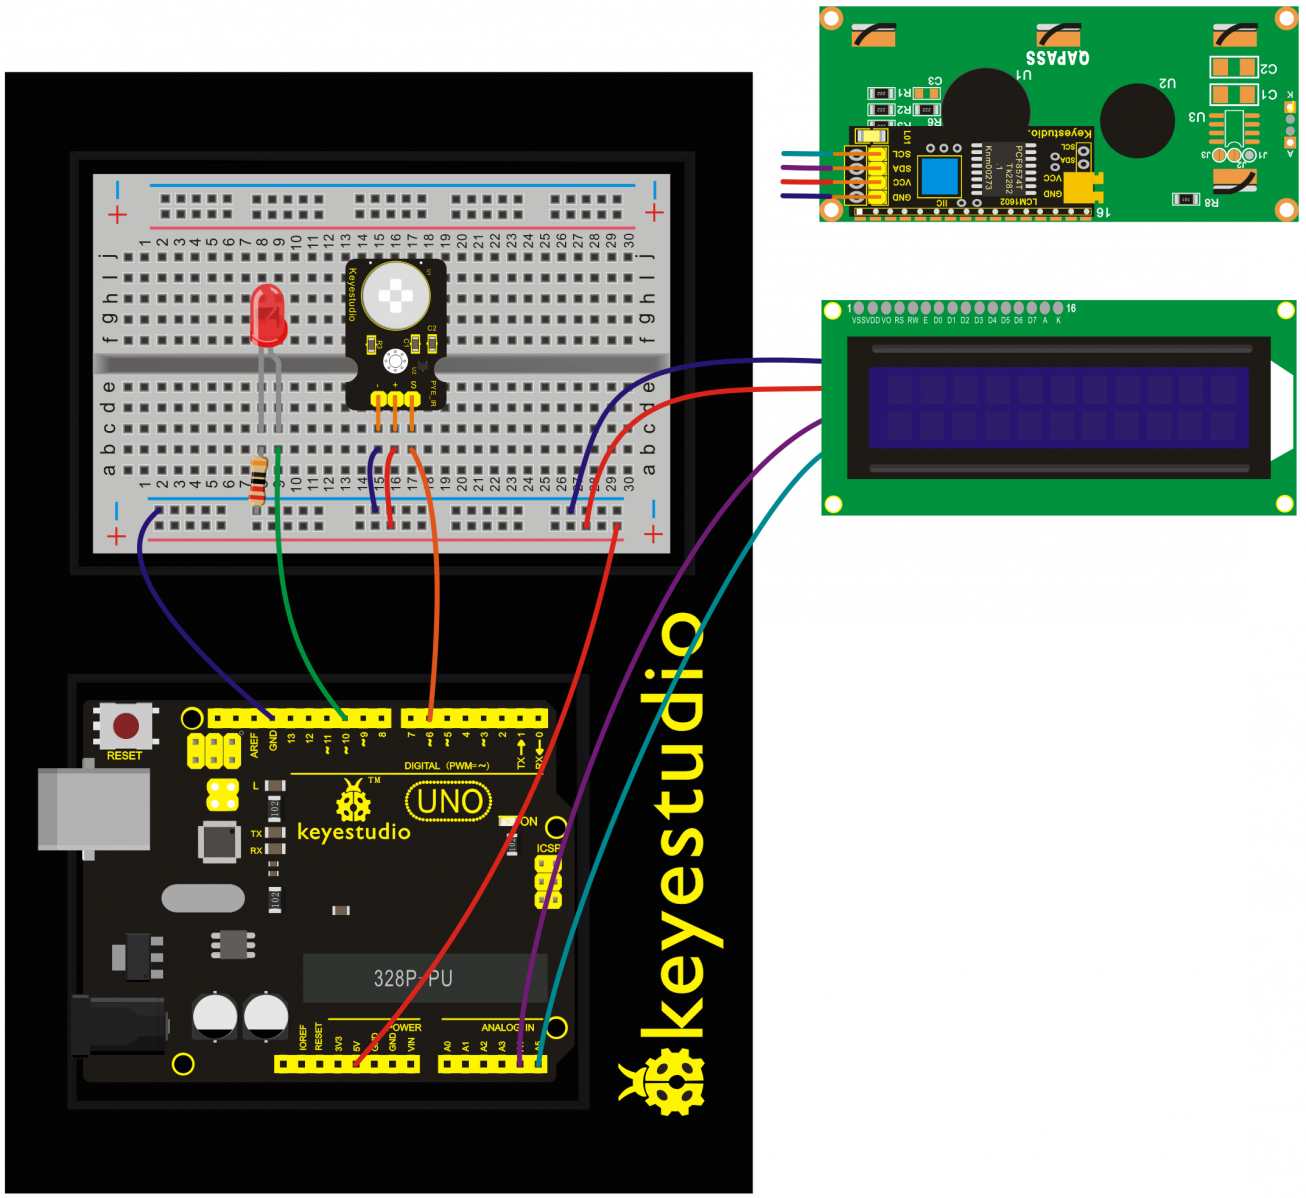
\includegraphics[width=\textwidth]{keyes_cablage_PIR_LCD_LED}
\caption{Montage à réaliser et tester}
\label{montagePIR}
\end{center}
\end{figure}
%}}}


\newpage


\partie{Le capteur PIR : Passive Infrared Sensor} \\                      %{{{1

Le capteur de mouvement infrarouge pyroélectrique peut détecter les signaux infrarouges d'une personne en mouvement ou d'un animal en mouvement, et émettre des signaux de commutation. Il peut être appliqué à une variété d'occasions pour détecter le mouvement du corps humain. Les capteurs infrarouges pyroélectriques conventionnels nécessitent un détecteur infrarouge pyroélectrique, une puce professionnelle, un circuit périphérique complexe, donc la taille est plus grande, avec un circuit complexe, et une fiabilité inférieure. Nous utilisons ici un nouveau capteur de mouvement infrarouge pyroélectrique, spécialement conçu pour Arduino. Il utilise un capteur infrarouge pyroélectrique à corps numérique intégré, a une taille plus petite, une plus grande fiabilité, une consommation d'énergie inférieure et un circuit périphérique plus simple.

\begin{minipage}{.5\textwidth} %
\textbf{Spécifications}\\
Input Voltage: 3.3 ~ 5V, 6V Maximum \\
Working Current: 15 uA \\
Working Temperature: -20 to 85 \celsius \\
Output Voltage: High 3V, low 0V \\
Output Delay Time (High Level): About 2.3 to 3s \\
Detection Angle: 100 \degree \\
Detection Distance: 7 meters \\
Output Indicator LED (output HIGH --> ON) \\
Pin Limit Current: 100mA \\
Size: 30\*20mm \\
Weight: 4g \\
\end{minipage}
\begin{minipage}{.45\textwidth} %
\begin{center}
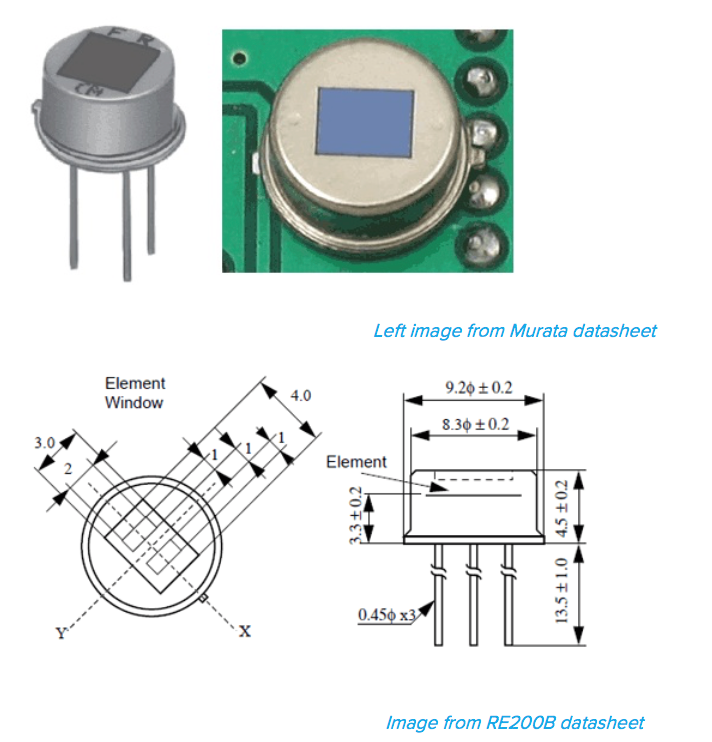
\includegraphics[width=\textwidth]{PIR_principle}
\end{center}
\end{minipage}

\begin{figure}[!h]
\begin{center}
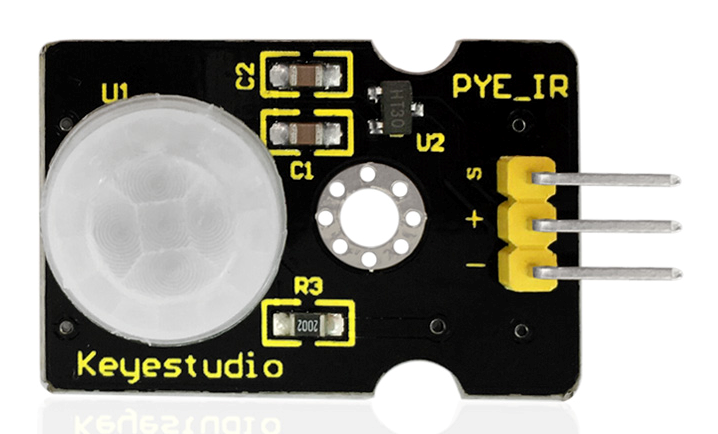
\includegraphics[width=0.5\textwidth]{keyesPIR}
\caption{Le capteur PIR déjà monté sur une carte fourni}
\end{center}
\end{figure}

\question Quel est est la tension d'alimentation ?
\reponse

\question Quel est est la consommation ?
\reponse

\question Quelle sont les valeurs de sortie quand quelque chose est détecté et sinon ?
\reponse

\question Pour la sortie à haut potentiel, quel sera le courant débité lorsque la sortie de la carte est directement branchée à une GPIO de la carte arduino ? \footnote{https://www.arduino.cc/en/Tutorial/DigitalPins}
\reponse

\question Pour la sortie à haut potentiel, est-ce que la carte PIR est capable d'allumer une LED ? Si oui, le faire.
\reponse
\tcbox{\textbf{Constatation professeur :} \hspace{5cm} } % package tcolorbox

\question Pour la sortie à haut potentiel, quel sera le courant débité ? \footnote{https://www.arduino.cc/en/Tutorial/DigitalPins}
\reponse

\question Dans la datasheet du BISS0001, l'example d'application montre que la broche S du composant optique est branché à une broche du BISS0001. Laquelle ?
\reponse


%}}}


\bigskip


\partie{Détection de proximité et affichge sur le LCD} \\                      %{{{1
\begin{figure}[p]
\begin{center}
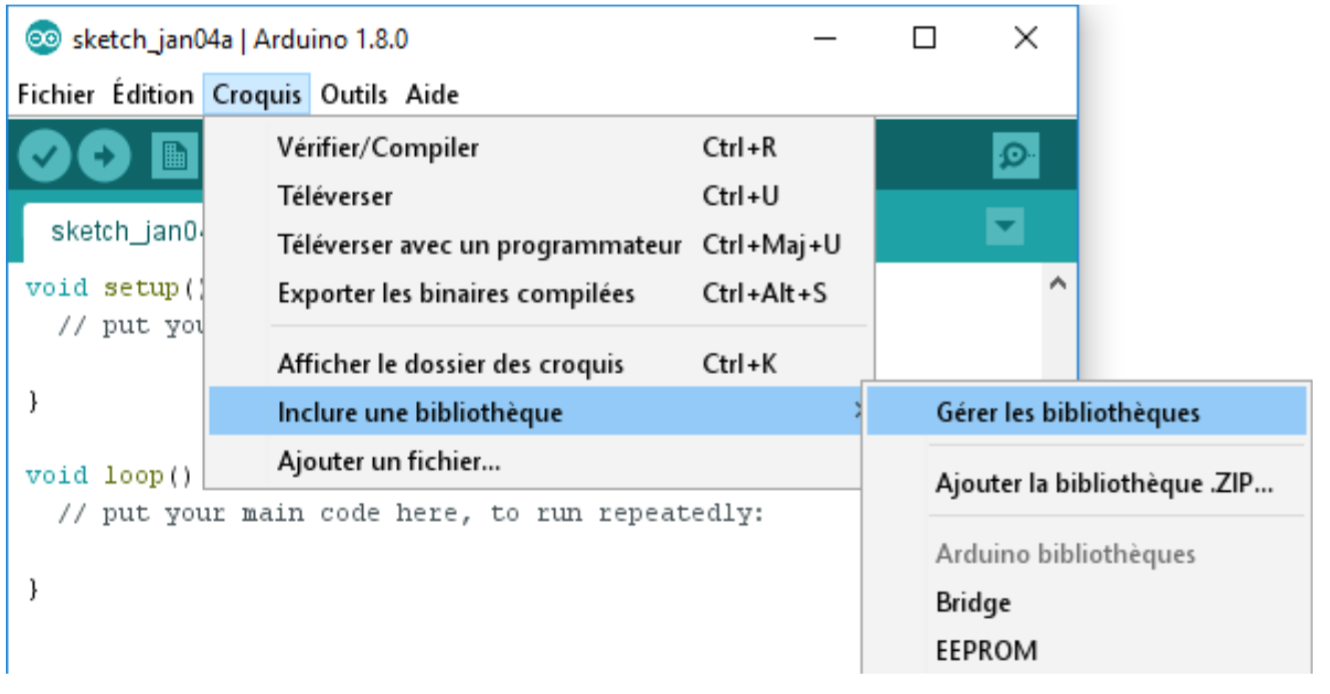
\includegraphics[width=0.9\textwidth]{bibliotheque_menu}
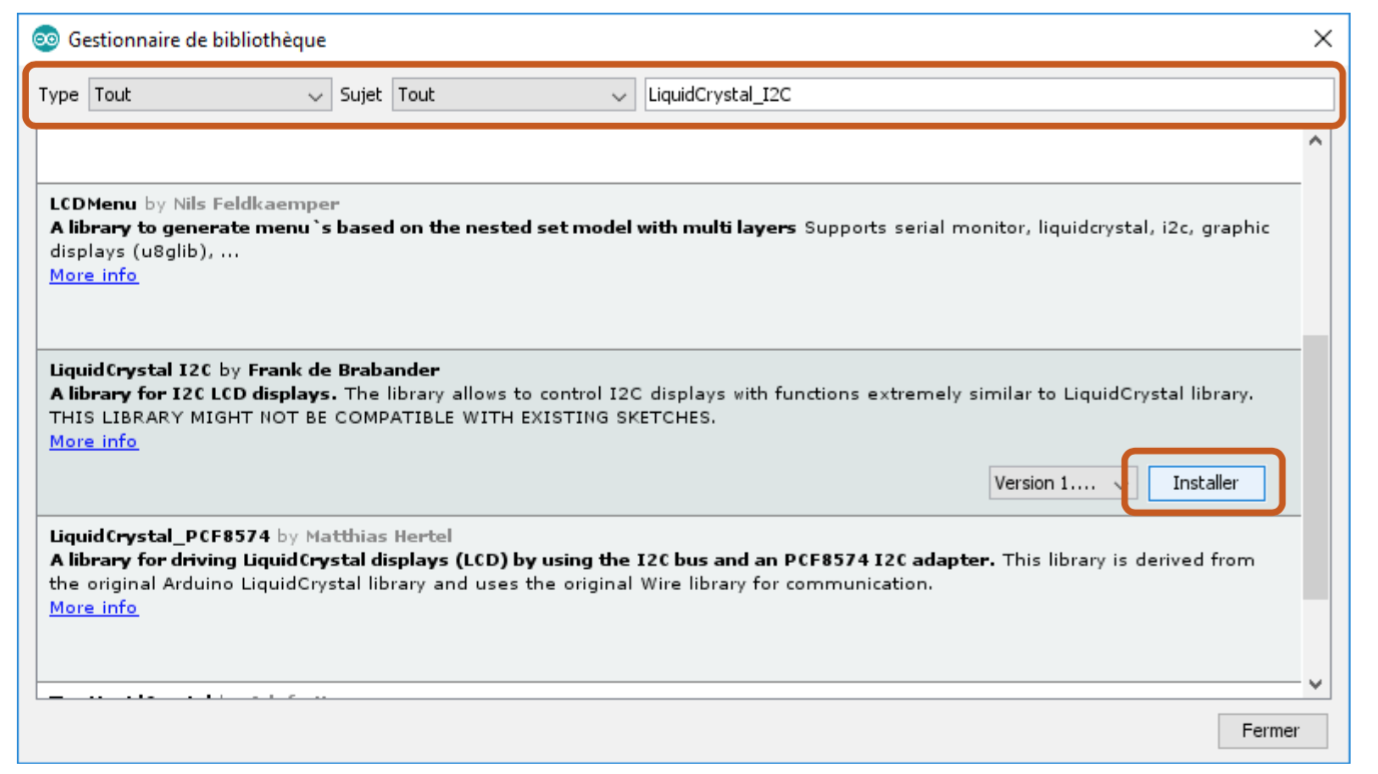
\includegraphics[width=0.9\textwidth]{bibliotheque_recherche}
\caption{Téléchargement et inclusion d'une librairie dans le logiciel arduino}
\end{center}
\end{figure}


\question Implémentez le montage de la figure \ref{montagePIR} et le code source suivante :
\begin{lstlisting}
#include <Wire.h>
#include <LiquidCrystal_I2C.h>
LiquidCrystal_I2C lcd(0x27,16,2);
byte sensorPin = 6;
byte indicator = 10;
void setup() {
  // initialize the lcd
  lcd.init();
  lcd.init();
  // Print a message to the LCD.
  lcd.backlight();
  pinMode(sensorPin,INPUT);
  pinMode(indicator,OUTPUT);
  Serial.begin(9600);
}

void loop() {
  byte state = digitalRead(sensorPin);
  digitalWrite(indicator,state);
  if(state == 1) {
    lcd.setCursor(2,0);
    lcd.print("quelqu un est");
    lcd.setCursor(2,1);
    lcd.print("est par la.");
  }
  else if(state == 0) {
    lcd.setCursor(2,0);
    lcd.print("No one!      ");
    lcd.setCursor(2,1);
    lcd.print("No one!      ");
    delay(500);
  }
}
\end{lstlisting}

\tcbox{\textbf{Constatation professeur :} \hspace{5cm} } % package tcolorbox

\question Quel le type des variables sensorPin et indicator ?
\reponse

\question Combien de fils connectent l'écran LCD ?
\reponse
\question Quels sont leur nom ?
\reponse
\question Pourrait-on connecter d'autres composants ?
\reponse
\question Que veut dire I2C ?
\reponse
\question Quel est le compromis majeur ?
\reponse


\question Que sont \texttt{<Wire.h> et <LiquidCrystal\_I2C.h>} ? \footnote{https://fr.wikipedia.org/wiki/Bibliothèque\_logicielle}
\reponse
\question A quoi servent-elles ?
\reponse
\question Comment le preprocessur gère t'il la commande \texttt{\#include} ? \footnote{https://fr.wikibooks.org/wiki/Programmation\_C/Préprocesseur\#Inclusion\_de\_fichiers}
\reponse

\question Quel est le type de la variable lcd ? \footnote{https://fr.wikipedia.org/wiki/Programmation\_orientée\_objet}
\reponse
\question Quel est ce type de programmation ?
\reponse
\question A quoi s'oppose t'il le plus souvent ?
\reponse

\question Donnez quelques méthodes de l'objet lcd.
\reponse
\reponse
\reponse
\reponse

\question Décrire l'algorithme
\reponse
\reponse
\reponse
\reponse
\reponse
\reponse
\reponse
\reponse

%}}}



\end{document}
%vim:fdm=marker

